\section{Mersenne Primes}
\theoremstyle{definition}
\begin{definition}{\textbf{Mersenne Prime}}
We call $p \in \N$ a Mersenne prime if $p$ is a prime number and $\exists n \in \N$ such that $p = 2^n - 1$ and $n$ is prime.
\end{definition}

\paragraph{}
We note that not all integers of the form $2^n -1, n \in \N$ are prime numbers. A simple counterexample would be that $2^4 - 1 = 15 = 3 \times 5$ is not a prime number. We therefore rely on a known table of Mersenne primes $p$ and their exponents $n$, such as Table A000043 in \cite{sloane2008line}.

\section{Bitstrings}

\paragraph{}
Throughout this report, we let $\mathcal{B}_n = \F_2^n - \{1^n\}$ be defined for every $n$ for which $2^n -1$ is a Mersenne prime. We define the following bijection:
\begin{align*}
    \mu &: \mathcal{B}_n \rightarrow \F_{2^n-1}\\
    \mu &= (x_1, \dots, x_n) \mapsto \sum_{i=1}^n 2^{i-1} x_i
\end{align*}

\paragraph{}
We sometimes write an element $x \in \mathcal{B}_n$ by its bit representation $x_n \dots x_1$ in big-endian order, where each $x_i \in \{0, 1\}$. In such situations, we will also use $b^k$ to denote the $k$-bit string of all $b$s, where $b \in \{0, 1\}$ and $k \in \N_{\leq n}$.

\subsection{Identification of $\mathcal{B}_n$ with $\F_{2^n -1}$}

\theoremstyle{definition}
\begin{definition}{\textbf{Addition and Multiplication on $\mathcal{B}_n$}}\label{add-mul-bits}
We define the addition and multiplication operators on $\mathcal{B}_n$ the following way:
\begin{align*}
    \forall a, b \in \mathcal{B}_n\:&[a + b = \mu^{-1}(\mu(a) + \mu(b))]\\
    \forall a, b \in \mathcal{B}_n\:&[a * b = \mu^{-1}(\mu(a) * \mu(b))]
\end{align*}
\end{definition}

\paragraph{}
We note that $2^n - 1$ is prime (by requirement that it be a Mersenne prime), so $\F_{2^n - 1}$ is a field with the usual addition and multiplication modulo $2^n - 1$. Letting the additive and multiplicative identities in $\mathcal{B}_n$ be $0^n$ and $0^{n-1} 1$ respectively, we then see that $\mu$ induces a ring structure on $\mathcal{B}_n$ (with the addition and multiplication operators from Definition \ref{add-mul-bits}) and is itself a ring isomorphism between $\mathcal{B}_n$ and $\F_{2^n - 1}$.

\paragraph{}
Therefore, $\mathcal{B}_n$ and $\F_{2^n - 1}$ are isomorphic as fields and we can use their elements and (addition and multiplication) operators interchangeably from this point onwards without making a distinction between them. We will henceforth rarely use $\mu$ explicitly (mostly to avoid confusing it with the mean of a random variable), though it should be clear from context when used.

\paragraph{}
We can perform addition in $\mathcal{B}_n$ in $O(n)$ by the association above, since addition of two $n$-bit numbers modulo $2^n - 1$ can be performed in $O(n)$. We can perform multiplication in $\mathcal{B}_n$ in $O(n \log{n} \log{\log{n}})$ using the algorithm given in \cite{schonhage1971schnelle}.

\subsection{Bit Operations in $\mathcal{B}_n$}

\theoremstyle{definition}
\begin{definition}
We define the following cyclic bit shift operators $s_\mathcal{L}$ and $s_\mathcal{R}$ the following way:
\begin{align*}
    s_\mathcal{L}(x_n \dots x_1) &= x_{n-1} \dots x_1 x_n\\
    s_\mathcal{R}(x_n \dots x_1) &= x_1 x_n \dots x_2
\end{align*}
\end{definition}

\begin{lemma}
Let $x \in \mathcal{B}_n$. Then $\mu(s_\mathcal{L}(x)) = \mu(a) \times 2$ and $\mu(s_\mathcal{R}(x)) = \mu(a) \times 2^{-1}$.
\end{lemma}
\begin{proof}
Write $x \in \mathcal{B}_n$ as $x_n \dots x_1$. There are two cases: $x_n = 0$ and $x_n = 1$.
Suppose $x_n = 0$. Then:
\begin{align*}
    \mu(x_n \dots x_1) \times 2 &= x_{n-1} 2^{n-1} + \dots + x_1 2^1\\
    &= \mu(x_{n-1} \dots x_1 0)\\
    &= \mu(x_{n-1} \dots x_2 x_n)\\
    &= \mu(s_\mathcal{L}(x_n \dots x_1))
\end{align*}
Suppose $x_n = 1$. Then:
\begin{align*}
    \mu(x_n \dots x_1) \times 2 &= x_n 2^n + x_{n-1} 2^{n-1} + \dots + x_1 2^1\\
    &= 1 + x_{n-1} 2^{n-1} + \dots + x_1 2^1\\
    &= x_n 2^0 + x_{n-1} 2^{n-1} + \dots + x_1 2^1\\
    &= \mu(x_{n-1} \dots x_1 0)\\
    &= \mu(x_{n-1} \dots x_1 x_n)\\
    &= \mu(s_\mathcal{L}(x_n \dots x_1))
\end{align*}
This proves that $\mu(s_\mathcal{L}(x)) = \mu(a) \times 2$. Since $s_\mathcal{R}$ is the inverse operation of $s_\mathcal{L}$, it holds that $\mu(s_\mathcal{R}(x)) = \mu(a) \times 2^{-1}$.
\end{proof}

\paragraph{}
We can now associate the operation $a \mapsto a \times 2^k$, for $k \in \N, a \in \F_{2^n - 1}$ with the operation $s_\mathcal{L}^k$ and associate the operation $a \mapsto a \times 2^{-k}$ with $s_\mathcal{R}^k$. This association makes it possible to perform $a \mapsto a \times 2^{\pm k}$ on $\F_{2^n - 1}$ in amortised $O(1)$ by cyclic bit shifting.

\theoremstyle{definition}
\begin{definition}
For any $x, y \in \mathcal{B}_n$, define $a \oplus b$ to be the sum of $a$ and $b$ regarded as elements of the vector space $\F_2^{n}$ over the field $\F_2$ (i.e. the bitwise exclusive-or operation).
\end{definition}

\paragraph{}
We note that the $\oplus$ operation on $\mathcal{B}_n$ can clearly be performed in $O(n)$.

\subsection{Hamming Weight}

\theoremstyle{definition}
\begin{definition}
Let $x = x_n \dots x_1 \in \mathcal{B}_n$. Then the \textit{Hamming weight} of $x$ is the cardinality of the set $\{i \in \Z_n: x_i = 1 \}$.
\end{definition}

Throughout this report, we define $\ham_h^n \subseteq \mathcal{B}_n$ to be the set of all bitstrings in $\mathcal{B}_n$ with Hamming weight $h$.

\begin{lemma}
Suppose $A, B \in \mathcal{B}_n$. Then the following hold:
\begin{align*}
    Ham(A + B) &\leq Ham(A) + Ham(B)\\
    Ham(A * B) &\leq Ham(A) * Ham(B)
\end{align*}
\end{lemma}

\paragraph{}
The above lemma is given as Lemma 2 in \cite{aggarwal2018new} and proven there.

\section{Statistics}

\begin{definition}{\textbf{Normal Distribution}}
We say that a random variable follows a normal distribution with mean $\mu$ and variance $\sigma^2$, written $X \sim N(\mu, \sigma^2)$ if the probability mass function $f_X$ is given by:
\begin{align*}
    f_X(x) = \frac{1}{\sqrt{2 \pi} \sigma} \exp{(-\frac{(x - \mu)^2}{2 \sigma^2})}
\end{align*}
\end{definition}

\begin{lemma}{\textbf{Gaussian Tail Bound}}
Let $X \sim N(\mu, \sigma^2)$. Then:
\begin{align}
    \Pr[|X - \mu| > t] &\leq 2 \exp{(-\frac{t^2}{2 \sigma^2})}\\
    \Pr[X - \mu > t] &\leq \exp{(-\frac{t^2}{2 \sigma^2})}\\
    \Pr[X - \mu < -t] &\leq \exp{(-\frac{t^2}{2 \sigma^2})}
\end{align}
\end{lemma}

\paragraph{}
The Gaussian tail bound (2.1) is a slightly looser version of Lemma 2.1 in \cite{samorodnitsky1991probability}. (2.2) and (2.3) are one-sided versions, derived from the fact that the normal distribution is symmetric about the mean.

\section{Security}

\paragraph{}
We give some important security definitions, most of which will be used in Chapter \ref{description_chapter}.

\theoremstyle{definition}
\begin{definition}{\textbf{Advantage}}
Let $\mathcal{X}_0$ and $\mathcal{X}_1$ be probability distributions. Let $\mathcal{A}$ be a Turing machine which takes an input that is from one of the two probability distributions and attempts to output $b \in \{0, 1\}$ if the input is from $\mathcal{X}_b$. Let $X_0 \sim \mathcal{X}_0$ and $X_1 \sim \mathcal{X}_1$. We define the \textit{advantage} of $\mathcal{A}$ in distinguishing $X_0$ and $X_1$ by:
\begin{align*}
    Adv^\mathcal{A}(X_0, X_1) = |\Pr[\mathcal{A}(X_0) = 1] - \Pr[\mathcal{A}(X_1) = 1]|
\end{align*}
\end{definition}

\subsection{Public-Key Cryptosystems}

\theoremstyle{definition}
\begin{definition}{\textbf{Public Key Cryptosystem}}
A public key cryptosystem is defined as a tuple $(\mathcal{P}, \mathcal{C}, \mathcal{K}, \mathcal{E}, \mathcal{D})$, where:
\begin{itemize}
    \item $\mathcal{P}$ is the set of possible plaintexts.
    \item $\mathcal{C}$ is the set of possible ciphertexts.
    \item $\mathcal{K}$ is the set of possible keys, each of which has a private component and a public component.
    \item $\mathcal{E}$ is the set of encryption functions. Each encryption function $e_k$ depends on \underline{only the public component} of a key $k \in \mathcal{K}$ and transforms a plaintext in $\mathcal{P}$ to a ciphertext in $\mathcal{C}$. The encryption functions may take in more than just a plaintext from $\mathcal{P}$ as input; they may also take in other values that are meant to be uniformly and randomly chosen by the encryptor from their respective sets. This is meant for ensuring semantic security by introducing randomness into the encryption process.
    \item $\mathcal{D}$ is the set of decryption functions. Each decryption function $d_k$ depends on \underline{both the public and private components} of a key $k \in \mathcal{K}$ and transforms a ciphertext in $\mathcal{C}$ to a plaintext in $\mathcal{P}$.
\end{itemize}
\end{definition}

\paragraph{}
To avoid cumbersome definitions, we may choose to present $\mathcal{E}$ and $\mathcal{D}$ as encryption and decryption algorithms rather than sets of encryption/decryption functions. We also let $pub(\mathcal{K})$ and and $pri(\mathcal{K})$ be the set of public keys and private keys respectively in $\mathcal{K}$. Each cryptosystem has an associated security parameter $\lambda$, which represents the difficulty of breaking the cryptosystem.

\paragraph{}
We now proceed to define two notions of security for public key cryptosystems. Consider the following game between a probabilistic polynomial-time adversary and a challenger:

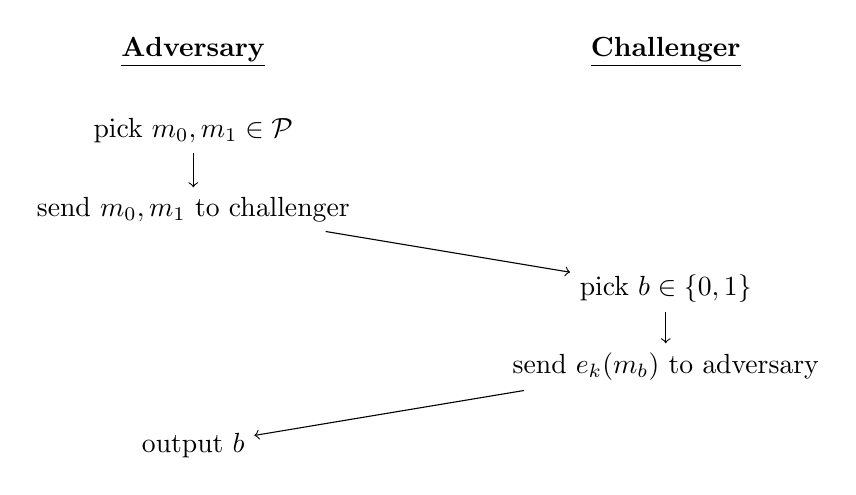
\begin{tikzpicture}
\node[] at (2, 49) {\underline{\textbf{Adversary}}};
\node[] at (8, 49) {\underline{\textbf{Challenger}}};
\node[](3) at (2, 48) {pick $m_0, m_1 \in \mathcal{P}$};
\node[](4) at (2, 47) {send $m_0, m_1$ to challenger};
\node[](5) at (8, 46) {pick $b \in \{0,1\}$};
\node[](6) at (8, 45) {send $e_k(m_b)$ to adversary};
\node[](7) at (2, 44) {output $b$};
\draw[->] (3) -- (4);
\draw[->] (4) -- (5);
\draw[->] (5) -- (6);
\draw[->] (6) -- (7);
\end{tikzpicture}

\paragraph{}
We define two kinds of security: ciphertext indistinguishability under chosen plaintext attack (IND-CPA) and ciphertext indistinguishability under chosen ciphertext attack (IND-CCA). Both have to do with how well an adversary guesses the correct $b$ in the game illustrated above, but differ what information the adversary is allowed to access in the process of playing the game.

\paragraph{}
Suppose the encryption functions are of the form $e_k: \mathcal{P} \times A \rightarrow \mathcal{C}$, where $A$ is the set over which some values are picked uniformly and randomly during encryption. Let $\mathcal{X}_{m_0, m_1}$ (resp. $\mathcal{Y}_{m_0, m_1}$) be the set of possible information available to the adversary who picked $m_0, m_1$ in the above game, in the case where the challenger chooses $b = 0$ (resp. $b = 1$).
\begin{align*}
\mathcal{X}_{m_0, m_1} &= \{ (m_0, m_1, e_k(m_0, a)) : a \in A \}\\
\mathcal{Y}_{m_0, m_1} &= \{ (m_0, m_1, e_k(m_1, a)) : a \in A \}\\
\end{align*}

\paragraph{}
Define two oracles:
\begin{itemize}
    \item $\mathcal{O}_k^\mathcal{E}$ is an encryption oracle that takes as input a plaintext $m \in \mathcal{P}$ and outputs a ciphertext $e_k(m, \dots)$, making uniform and random choices (the $\dots$ part) if required by the encryption algorithm
    \item $\mathcal{O}_k^\mathcal{D}$ is a decryption oracle that takes as input a ciphertext $c \in \mathcal{C}$ and outputs a plaintext $d_k(c)$
\end{itemize}

\paragraph{}
With these definitions in place, we can proceed to define IND-CPA and IND-CCA.

\theoremstyle{definition}
\begin{definition}{\textbf{IND-CPA}}
Let $\mathcal{A}$ be a probabilistic polynomial time adversary with access to $\mathcal{O}_k^\mathcal{E}$ who picked $m_0, m_1 \in \mathcal{P}$ in the game illustrated above. Let $X \sim \mathcal{U}(\mathcal{X}_{m_0, m_1})$ and $Y \sim \mathcal{U}(\mathcal{Y}_{m_0, m_1})$ be random variables. Then:
\begin{align*}
Adv^\mathcal{A}(X, Y) \in O(2^{-\lambda})
\end{align*}
\end{definition}

\theoremstyle{definition}
\begin{definition}{\textbf{IND-CCA}}
Let $\mathcal{A}$ be a probabilistic polynomial time adversary with access to $\mathcal{O}_k^\mathcal{D}$ who picked $m_0, m_1 \in \mathcal{P}$ in the game illustrated above. Let $X \sim \mathcal{U}(\mathcal{X}_{m_0, m_1})$ and $Y \sim \mathcal{U}(\mathcal{Y}_{m_0, m_1})$ be random variables. Then, provided the adversary does not query the oracle with the ciphertext sent by the challenger:
\begin{align*}
Adv^\mathcal{A}(X, Y) \in O(2^{-\lambda})
\end{align*}
\end{definition}

\paragraph{}
IND-CPA is equivalent to the notion of \textit{semantic security} and the two terms are often used interchangeably. In the definition of IND-CCA, if the adversary is allowed to adaptively choose ciphertexts to decrypt, it is called IND-CCA2; otherwise it is called IND-CCA1.

\subsection{Key Exchange Mechanisms}

\begin{definition}{\textbf{Key Exchange Mechanism}}
A key exchange mechanism is defined as a tuple $(\mathcal{P}, \mathcal{C}, \mathcal{K}, \overline{\mathcal{E}}, \overline{\mathcal{D}})$, where:
\begin{itemize}
    \item $\mathcal{P}$ is the set of possible plaintexts.
    \item $\mathcal{C}$ is the set of possible ciphertexts.
    \item $\mathcal{K}$ is the set of possible keys, each of which has a private component and a public component.
    \item $\overline{\mathcal{E}}$ is an \textit{encapsulation algorithm} that takes as input a public key, makes random choices (like the encryption algorithm in a public key cryptosystem) and outputs a pair $(C, K) \in \mathcal{C} \times \mathcal{P}$
    \item $\overline{\mathcal{D}}$ is a \textit{decapsulation algorithm} that takes as input both a private key and a ciphertext, and either outputs a plaintext or gives an error
\end{itemize}
\end{definition}

\paragraph{}
Following the definition in Subsection 2.2 of \cite{aggarwal2018new}, we call a key exchange mechanism $(1 - \delta)$-correct if, given a public key $k_{pub}$ and a corresponding private key $k_{pri}$, $\Pr[\overline{\mathcal{D}}(k_{pri}, C) = K | \overline{\mathcal{E}}(k_{pub}) = (C, K)] \geq 1 - \delta$.

\paragraph{}
We can give definitions of IND-CPA and IND-CCA for key exchange mechanisms as well following that given in \cite{aggarwal2018new}, with $\mathcal{O}_k^{\overline{\mathcal{E}}}$ and $\mathcal{O}_k^{\overline{\mathcal{D}}}$ being the encapsulation and decapsulation oracles respectively. Consider a fixed key $k \in \mathcal{K}$, which has a public component $k_{pub}$ and private component $k_{pri}$.

\theoremstyle{definition}
\begin{definition}{\textbf{IND-CPA}}
Let $\mathcal{A}$ be a probabilistic polynomial time adversary with access to $\mathcal{O}_k^{\overline{\mathcal{E}}}$. Let $X = (C, K_0) \sim \overline{\mathcal{E}}(k_{pub})$ and $Y = (C, K_1)$ where $K_1$ is uniformly and randomly sampled from $\mathcal{P}$. Then $Adv^\mathcal{A}(X, Y) \in O(2^{-\lambda})$.
\end{definition}

\theoremstyle{definition}
\begin{definition}{\textbf{IND-CCA}}
Let $\mathcal{A}$ be a probabilistic polynomial time adversary with access to $\mathcal{O}_k^{\overline{\mathcal{D}}}$. Let $X = (C, K_0) \sim \overline{\mathcal{E}}(k_{pub})$ and $Y = (C, K_1)$ where $K_1$ is uniformly and randomly sampled from $\mathcal{P}$. Then $Adv^\mathcal{A}(X, Y) \in O(2^{-\lambda})$, provided the adversary is not allowed to query the oracle with $C$.
\end{definition}

\section{Miscellaneous}

\theoremstyle{definition}
\begin{definition}{\textbf{Projection}}
Let $A$ be a set, $I$ be an indexing set and $B = A^{|I|}$. Then for all $i \in I$ let $\pi_i$ denote the projection onto the $i$th coordinate. That is, for all $b = \{a_j\}_{j \in I} \in B$, we have $\pi_i(b) = a_i$.
\end{definition}

\theoremstyle{definition}
\begin{definition}{\textbf{Randomness Extractor}}
Let $A$ and $B$ be sets. A randomness extractor (or extractor) is a function $Ext: A \rightarrow B$ such that $Ext(a)$ is indistinguishable from a uniformly and randomly chosen $b \in B$ for an adversary that does not know $a \in A$.
\end{definition}